\documentclass{article}
\usepackage{geometry}
\usepackage{graphicx}
\usepackage{float}
\geometry{
	a4paper,
	total={170mm,257mm},
	left=20mm,
	top=20mm
}

\begin{document}
	\section{Desain dan Implementasi Penambangan Data}
		\begin{figure}[H]
			\centering{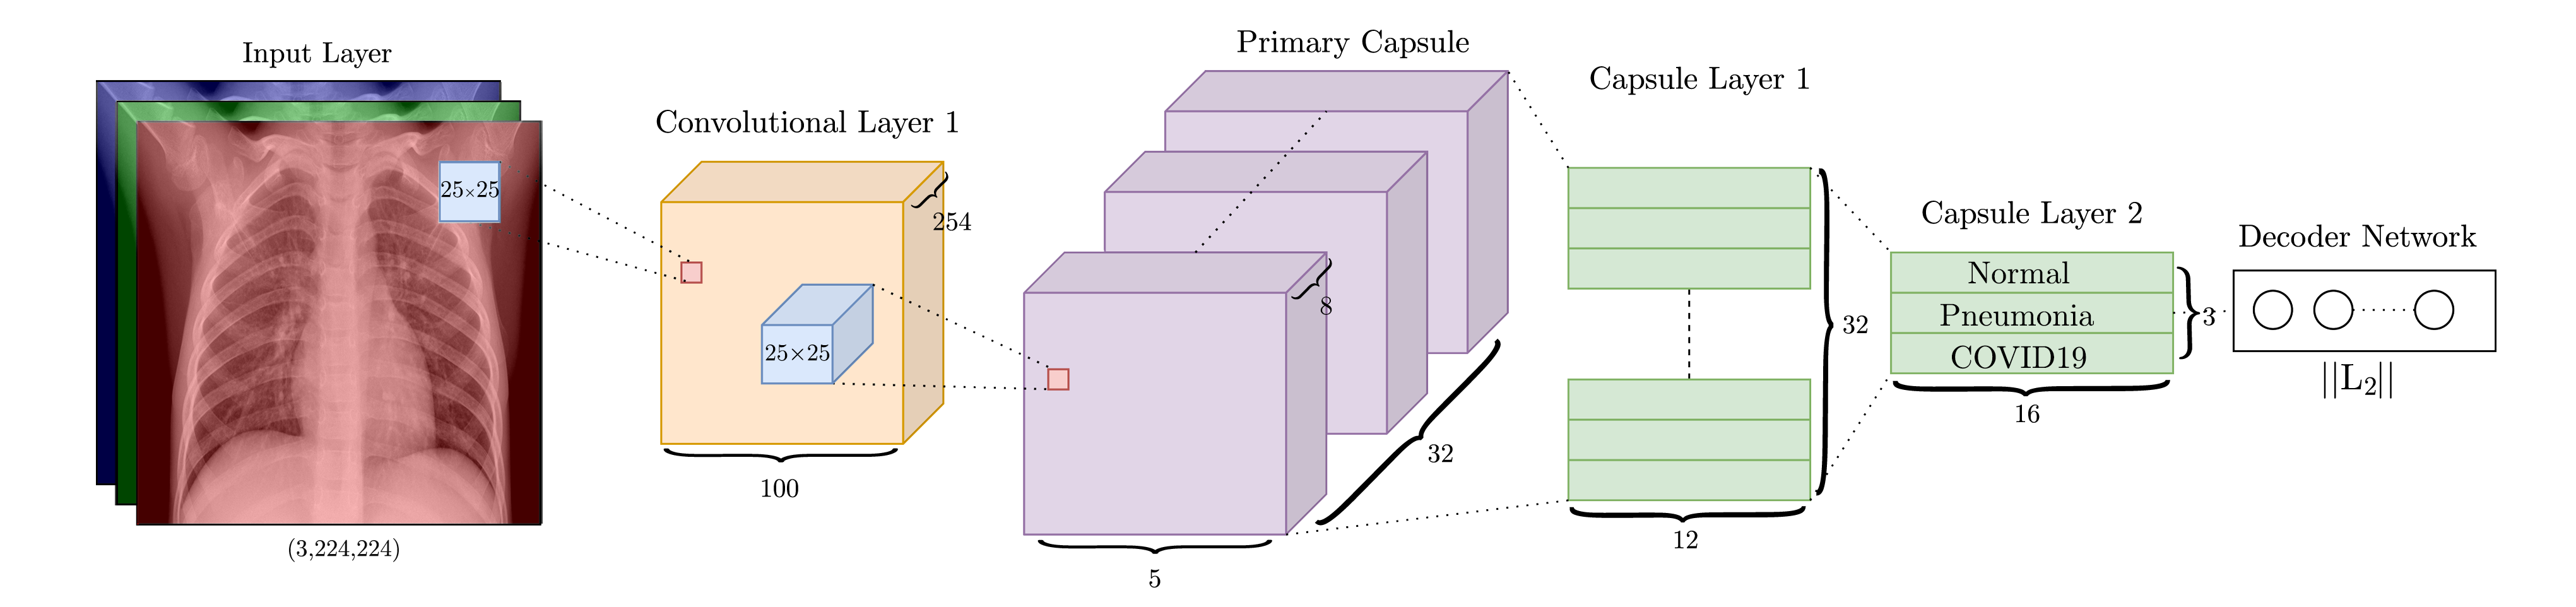
\includegraphics[width=\linewidth]{./images/arsitektur/arsitektur_fig1.png}}
			\caption{Arsitektur CapsNet}
			\label{arsitektur_1}
		\end{figure}
		\begin{figure}[H]
			\centering{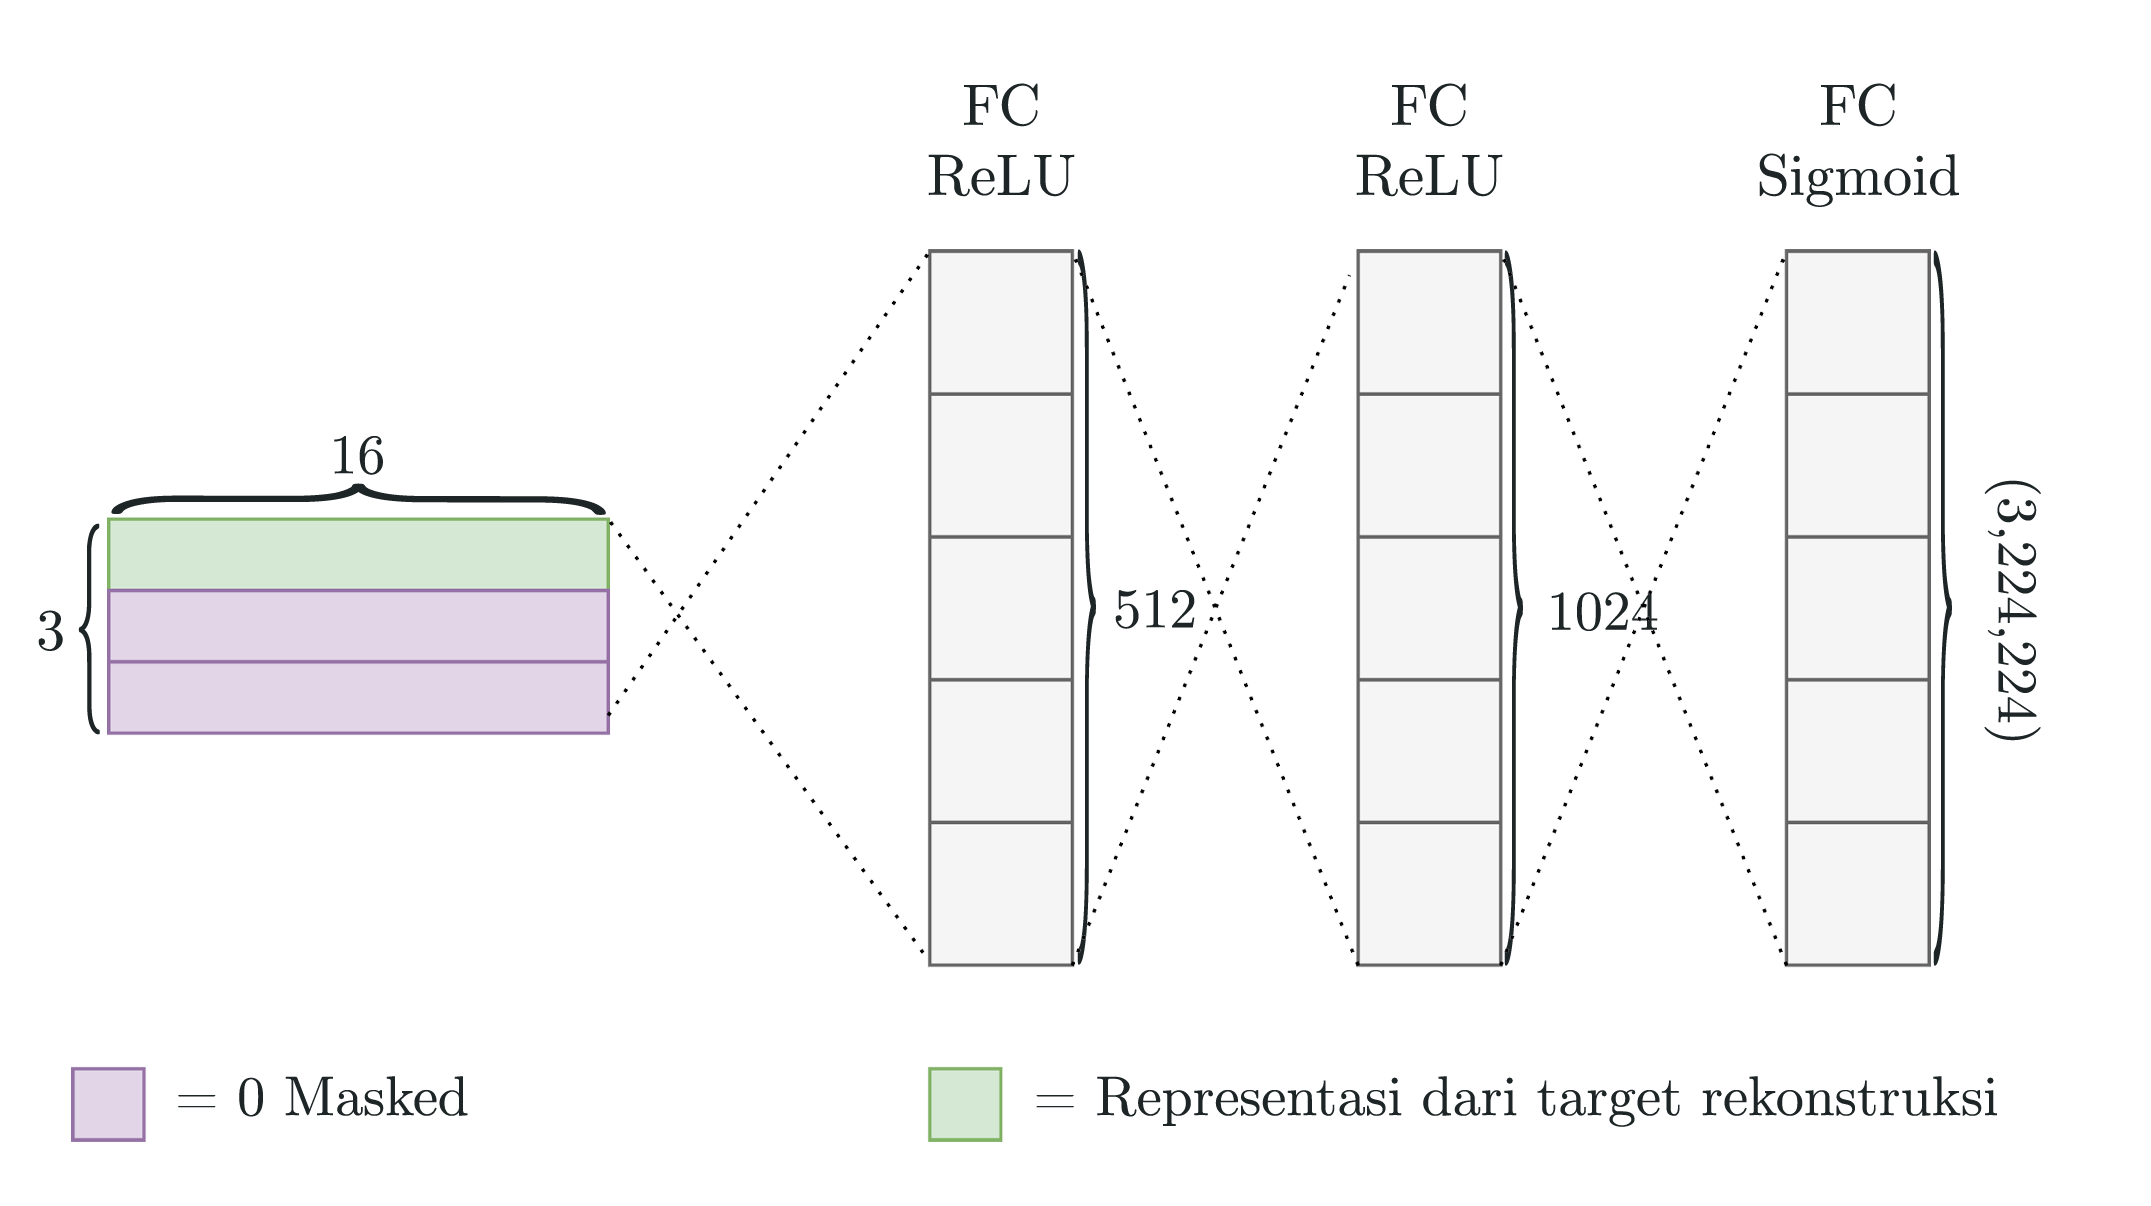
\includegraphics[width=300px, height=170px]{./images/arsitektur/arsitektur_fig2.png}}
			\caption{Arsitektur Decoder Network}
			\label{arsitektur_2}
		\end{figure}
		\subsection{Arsitektur CapsNet}
		Arsitektur CapsNet yang digunakan dalam makalah ini terdiri dari :
		\begin{enumerate}
			\item \textit{Input Layer}\\
			\textit{Input} menggunakan gambar berukuran 224x224 dengan 3 \textit{channel} yaitu \textit{channel red, green,} dan \textit{blue} atau biasa disebut dengan RGB.
			
			\item \textit{Convolutional Layer 1}\\
			\textit{Layer} ini akan melakukan operasi konvolusi pada gambar \textit{input} menggunakan \textit{out channel} atau \textit{filter} sebanyak 256 dengan \textit{kernel} berukuran 25x25 dan \textit{stride} sebanyak 2. Layer ini akan menghasilkan \textit{feature map}.
			
			\item \textit{Primary Capsule}\\
			\textit{Layer} ini akan mengubah hasil konvolusi menjadi \textit{capsule-capsule}. \textit{Layer} ini terdiri dari beberapa layer, yaitu:
			\begin{itemize}
				\item \textit{Convolution Layer 2}\\ 
				\textit{Layer} ini mendapatkan \textit{input channel} sebanyak 256, lalu operasi konvolusi pada \textit{layer} ini menggunakan \textit{out channel} sebanyak 256 dengan \textit{kernel} berukuran 25x25  dan \textit{stride} sebanyak 16.
				
				\item \textit{Reshape}\\
				Operasi reshape digunakan untuk mendapatkan \textit{capsule}.
				
				\item \textit{Squash}\\
				\textit{Layer squash} adalah \textit{layer} aktivasi dari primary capsule yang mengubah panjang vektor besar menjadi mendekati 1 dan vektor kecil menjadi 0.
			\end{itemize}
			
			\item \textit{Capsule Layer 1}\\
			\textit{Layer} ini mendapatkan \textit{input capsule} sebanyak 800 berdimensi 8 untuk setiap \textit{capsule}. Lalu algoritma \textit{Routing-by-agreement} akan dijalankan pada layer ini dan menghasilkan \textit{output capsule} sebanyak 32 berdimensi 12 untuk setiap \textit{capsule}.
			
			\item \textit{Capsule Layer 2}\\
			\textit{Layer} ini mendapatkan \textit{input capsule} sebanyak 32 berdimensi 12 untuk setiap \textit{capsule}. Lalu algoritma \textit{Routing-by-agreement} akan dijalankan pada layer ini dan menghasilkan \textit{output capsule} sebanyak jumlah \textit{class} yaitu 3 dan berdimensi 16 untuk setiap \textit{capsule}.
			
			\item \textit{Decoder Network}\\
			\textit{Decoder Network} adalah \textit{layer} yang digunakan CapsNet untuk menghitung \textit{loss} dan melakukan proses rekonstruksi gambar. \textit{Decoder Network} terdiri dari:
			\begin{itemize}
				\item \textit{Fully Connected Layer 1}\\
				\textit{Layer} ini mendapatkan \textit{input} sebanyak jumlah \textit{output capsule} dikali dimensi \textit{capsule} dari \textit{layer} sebelumnya yaitu 3x16 dan menghasilkan 512 \textit{output neuron}. Fungsi aktivasi yang digunakan pada layer ini adalah ReLu.
				
				\item \textit{Fully Connected Layer 2}\\
				\textit{Layer} ini mendapatkan \textit{input} sebanyak jumlah \textit{output neuron} dari \textit{layer} sebelumnya yaitu 512 dan menghasilkan 1024 \textit{output neuron}. Fungsi aktivasi yang digunakan pada layer ini adalah ReLu.
				
				\item \textit{Fully Connected Layer 3}\\
				\textit{Layer} ini mendapatkan \textit{input} sebanyak jumlah \textit{output neuron} dari \textit{layer} sebelumnya yaitu 1024 dan menghasilkan \textit{output neuron} sebanyak ukuran gambar \textit{input} yaitu 224x224x3. Fungsi aktivasi yang digunakan pada layer ini adalah \textit{sigmoid}.
			\end{itemize}
			
		\end{enumerate}
\end{document}
    